%! TeX program = lualatex
\documentclass[../main.tex]{subfiles}
\begin{document} 
\section{Vectors}

We have been looking at models involving one quantity, e.g., the population of a group of unicorns.  We now develop mathematical tools (\emph{linear} vector fields and \emph{linear} systems of differential equations) to model systems involving two or more quantities, e.g., an ecosystem involving a predator and prey.

We use an introductory example to demonstrate why vectors are useful in science.
\begin{example}
  Consider an ecosystem involving orcas (predators) and seals (preys). Their population over time (in years) is presented as a table. 

  \begin{table}[H]
    \centering
    \begin{tabular}{r|c|c|c|c}
      time  & \(0\) & \(1\) & \(2\) & \(3\)  \\\midrule
      orcas & \(5\) & \(6\) & \(4\) & \(3\)  \\
      seals & \(5\) & \(3\) & \(2\) & \(4\)  \\
    \end{tabular}
  \end{table}

  \begin{center}
    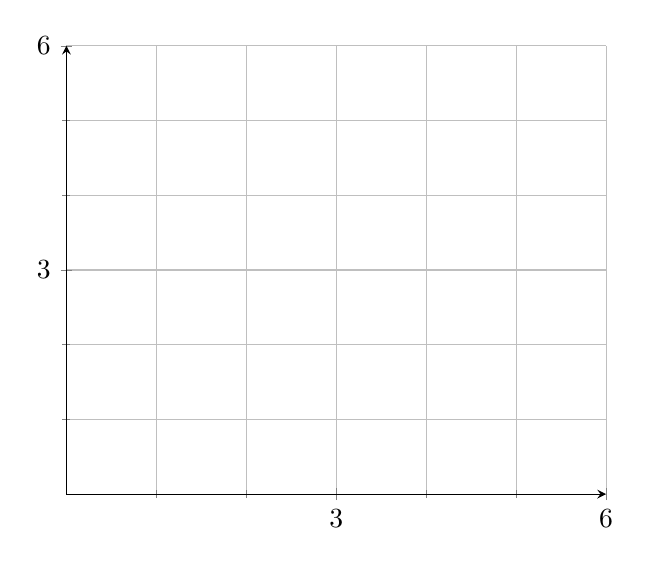
\begin{tikzpicture}[scale=1]
      \begin{axis}[xmin=0, xmax=6, ymin=0, ymax=6, enlargelimits, grid=both, minor tick num=2, axis lines=middle, xtick={0, 3, 6}, ytick={0, 3, 6}]
      \end{axis}
    \end{tikzpicture}
    \quad
    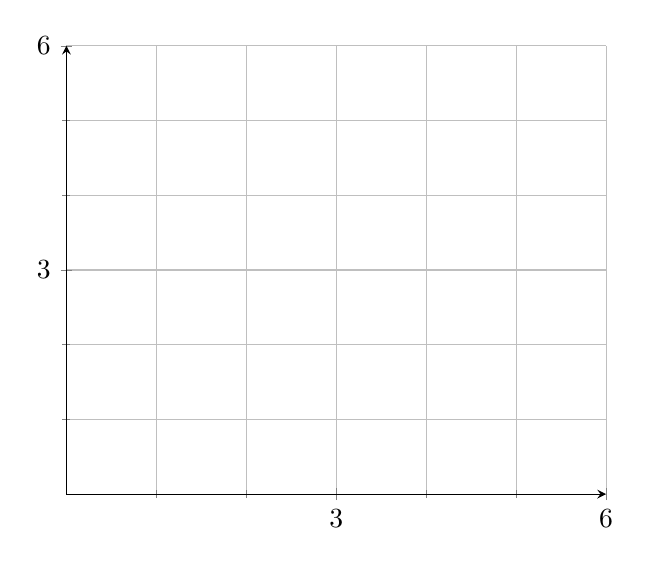
\begin{tikzpicture}[scale=1]
      \begin{axis}[xmin=0, xmax=6, ymin=0, ymax=6, enlargelimits, grid=both, minor tick num=2, axis lines=middle, xtick={0, 3, 6}, ytick={0, 3, 6}]
      \end{axis}
    \end{tikzpicture}
  \end{center}
\end{example}

\blanklines{8}

\begin{definition}[vectors]
  A (state) \hlmain{vector} \(\vec{x}\) is an ordered list of numbers
  \[
    \vec{x} = 
    \begin{bmatrix}
      x_{1} \\ x_{2} \\ \vdots \\ x_{n}
    \end{bmatrix}
    = 
    \begin{bmatrix}
      x_{1} & x_{2} & \cdots & x_{n}
    \end{bmatrix}^{T}.
  \]

  The number of rows in \(\vec{x}\) (zeros included) is called the \hlmain{dimension} of \(\vec{x}\).  Two vectors \(\vec{u}, \vec{v}\) are \hlmain{equal} if they have the same dimension and \(u_{1} = v_{1}, \ldots., u_{n} = v_{n}\).
\end{definition}
Depending on the application, a vector can be visualized as a point or as an arrow.

\clearpage

\section{Algebraic operations on vectors}

We now study vectors abstractly and quickly introduce all fundamental operations on vectors. \medskip

\begin{itemize}[wide]

  \item Every vector has a \hlmain{direction} and a \hlmain{length}. The direction is implicit, but the length \(\|\vec{v}\|\) is defined by the Pythagorean theorem:
    \begin{equation}
      \| \vec{v} \| = \sqrt{ (v_{1})^{2} + \cdots + (v_{n})^{2} }.
    \end{equation}
    \blanklines{5}

  \item We can multiply a \hlsupp{constant \(c\)} by a \hlmain{vector \(\vec{v}\)}, and \hlmain{add two vectors} having the same dimension.
    \begin{equation}
      \hlsupp{c}\, \hlmain{\vec{v}}
      = 
      \hlsupp{c}
      \begin{bmatrix}
        \hlmain{v_{1}} \\ \hlmain{v_{2}} \\ \vdots \\ \hlmain{v_{n}}
      \end{bmatrix}
      =
      \begin{bmatrix}
        \hlsupp{c}\, \hlmain{v_{1}} \\ \hlsupp{c}\, \hlmain{v_{2}} \\ \vdots \\ \hlsupp{c}\, \hlmain{v_{n}}
      \end{bmatrix}
      \quad\text{and}\quad
      \hlmain{\vec{u} + \vec{v}}
      =
      \begin{bmatrix}
        u_{1} \\ u_{2} \\ \vdots \\ u_{n}
      \end{bmatrix}
      +
      \begin{bmatrix}
        v_{1} \\ v_{2} \\ \vdots \\ v_{n}
      \end{bmatrix}
      =
      \begin{bmatrix}
        u_{1} + v_{1} \\ v_{2} + v_{2} \\ \vdots \\ u_{n} + v_{n}
      \end{bmatrix}.
    \end{equation}

    \blanklines{5}

    \includegraphics{../standalones/build/plot-RR2}
    \quad
    \includegraphics{../standalones/build/plot-RR2}
    \quad
    \includegraphics{../standalones/build/plot-RR2}

    \faStar{} In the operation \(c \, \vec{v}\), the constant \(c\) is called a \hlmain{scalar} because it stretches (aka scales) a vector's length without rotation.  The length of the stretched vector \(c \, \vec{v}\) is \underline{\hspace{2in}\phantom{\huge X}}.

  \item The \hlmain{dot product} \(\vec{u} \bullet \vec{v}\) takes two vectors of the same dimension as input and outputs a scaler. 
    \begin{equation}
      \vec{u} \bullet \vec{v} = u_{1} v_{1} + \cdots + u_{n} v_{n}.
    \end{equation}
    
    \blanklines{5}
\end{itemize}

A \hlmain{matrix} is an \(m\)-by-\(n\) array of numbers where \(m\) is the number of rows and \(n\) is the number of columns.  Moreover, if \(A\) is a matrix, then we write \(A_{ij}\) to represent the number in the \(i\)-th row and \(j\)-th column of the matrix \(A\). 
\blanklines{5}

We can multiply an \(m\)-by-\(n\) matrix \(A\) by a \(n\)-dimensional vector \(\vec{v}\) to produce an \(n\)-dimensional vector \(\vec{u} = A\vec{v}\) whose entries are defined by
\[
  u_{i} = A_{i1} v_{1} + \cdots + A_{in} v_{n} 
  \quad\text{for each row index \(i = 1, \ldots, n\)}.
\]
\blanklines{5}

% The number of columns in \(A\) \hlwarn{must match} the number of rows in \(\vec{v}\).  Matrix-vector multiplication is defined by 

We can multiply an \(m\)-by-\(n\) matrix \(A\) by an \(n\)-by-\(k\) matrix \(B\) to produce an \(m\)-by-\(k\) matrix \(C = AB\) whose entries are defined by
% The number of columns in \(A\) must match the number of rows in \(B\). 
\begin{equation}
  C_{ij} = 
  A_{i1} B_{1j} + A_{i2} B_{2j} + \cdots + A_{in} B_{nj}
  \quad\text{for each \(i = 1, \ldots, m\) and each \(j = 1, \ldots, k\)}.
\end{equation}

\blanklines{10}
Matrices are functions that take vector as inputs and output vectors (of the same dimension). More on this tomorrow. For now, we must remember that matrix-matrix multiplications are actually function compositions so we can correctly perform the operation \(A B \vec{v}\):
\blanklines{10}
\clearpage

We work with vectors more or less as if they were regular numbers. 

\begin{example}
  Find the vector \(\vec{x}\) in the equation \(\begin{bmatrix} 1 \\ 3 \end{bmatrix} + 2 \vec{x} = \begin{bmatrix} -3 \\ 5 \end{bmatrix}\) and calculate \(\| -5 \vec{x} \|\).

  \blanklines{10}
\end{example}

\begin{example}
  Let \(\vec{x} = [ x_{1} \; x_{2} \; x_{3} ]^{T}\).  Write \(-3x_{1} + x_{2} - 3x_{3}\) as a dot product. 

  \blanklines{5}
\end{example}

\begin{example}
  Let \(\vec{x} = [ x_{1} \; x_{2} \; x_{3} ]^{T}\).  Write \(- x_{1} + \tfrac{1}{2}x_{3}\) as a dot product. 
  
  \blanklines{5}
\end{example}

\begin{example}
  Perform the calculation \(A^{2} \vec{v}\) given that \(A = \begin{bmatrix} 1 & 2 \\ 0 & -1 \end{bmatrix}\) and \(\vec{v} = \begin{bmatrix} 1 \\ 1/2 \end{bmatrix}\).
  \blanklines{5}
\end{example}

\begin{example}
  Perform the calculation \(A^{3} \vec{v}\) given that \(A = \begin{bmatrix} 4 & 0 \\ 0 & -5 \end{bmatrix}\) and \(\vec{v} = \begin{bmatrix} 1 \\ -1 \end{bmatrix}\).
  \blanklines{5}
\end{example}

\begin{example}
  Consider the equation \(\vec{u} \bullet \vec{v} = 4\). What is \(\|\vec{u}\|\) if \(\vec{v} = \left(\tfrac{1}{\sqrt{2}}, \tfrac{1}{\sqrt{2}}\right)\) and the angle between them is \(\pi/6\)?

  \blanklines{10}
\end{example}

For completeness, here is a frequently used terminology in the study of vectors.

A linear combination of (finitely many) vectors \(\vec{u}, \vec{v}, \vec{w}, \ldots\) is a mix of scaling and additions:
\[
  a \vec{u} + b \vec{v} + c \vec{w} + \cdots, \text{ where \(a,b,c, \ldots\) are scalers}.
\]

Also for completeness, we can take two vectors \(\vec{u}, \vec{v}\) and define a third vector called their cross product 
\[
  \vec{u} \times \vec{v} = 
  \begin{bmatrix}
    u_{2} v_{3} - u_{3} v_{2} \\
    - u_{1} v_{3} + u_{3} v_{1} \\
    u_{1} v_{2} - u_{2} v_{1} \\
  \end{bmatrix}.
\]

For more details of the cross product, see pages 149 to 151 of the textbook. 

\end{document}
